\documentclass{acmtog} % V1.2

\usepackage[hypertexnames=false, pdftex]{hyperref}
\hypersetup{ colorlinks = true, linkcolor = black, urlcolor = blue, citecolor = blue }
\usepackage{float}
\let\oldquote\quote
\let\endoldquote\endquote
\renewenvironment{quote}[2][]
  {\if\relax\detokenize{#1}\relax
     \def\quoteauthor{#2}%
   \else
     \def\quoteauthor{#2~---~#1}%
   \fi
   \oldquote}
  {\par\nobreak\smallskip\hfill(\quoteauthor)%
   \endoldquote\addvspace{\bigskipamount}}

\acmVolume{1}
\acmNumber{1}
\acmYear{2018}
\acmMonth{March}
\acmArticleNum{1}
\makeatletter
\def\runningfoot{\def\@runningfoot{}}
\def\firstfoot{\def\@firstfoot{}}
\makeatother


\begin{document}

\markboth{Experimental Sentiment Analysis on Twitter}{A Real Time Stream and Big Data Process}

\title{Sentiment Analysis on Twitter : Effects in a Social Network} % title

\author{Mohamed Ben Hamdoune {\upshape and} Yannis Tannier
\affil{University of Paris-Descartes}
}

\category{H.2.8}{Database Applications}{Big Data and Real Stream}[Cloud Computing]
\category{I.3.7}{Learning}{Apache Spark and Hadoop}[Social Media Analytics]

\terms{Twitter, Psychological Profile}

\keywords{Data Mining, Natural Languages Processing, Sentiment Analysis, Classification, Text Mining}

\acmformat{Mohamed Ben Hamdoune, Yannis Tannier. 2018. Sentiment Analysis for Twitter : Effects in a Social Network.}

\maketitle

\begin{bottomstuff}
Jason Scott Sadofsky acknowledges a Jason Scott, is an American archivist, historian of technology, and film-maker. Archive Team is a group dedicated to preserving digital history that was founded by Jason Scott in 2009. Data was collected from the website of The Archive Team.

\end{bottomstuff}


\begin{abstract}

Our purpose is to build a powerful platform for real-time data analysis of tweets on twitter trends. We also want to analyse all the tweets of 2017 based on a downloaded sample of data (average of 6 To). All this data analysis will be accessible via a web interface that will be developed. We want to build a powerful system of sentiments analysis by making a database structure of tweets which is relevant about impacts and effects. The system should provide a faster way to execute Machine Learning methodologies behind data extracted from Twitter. Analysis news actuality by getting an analysis on actual trends with real stream data by building an efficient web interface to get results easily and build a system without false accounts and keep a control on data continuously.
\end{abstract}

\section{Introduction}

The main subject is Sentiment Analysis on Twitter\footnote{\url{https://twitter.yannistannier.io/#/dashboard}}, a microblogging platform where people can easily share their thought on anything and their habits too. We have a lot of publications on sentiment analysis but not so much research about impacts and their effect on society. The maximum characters are 140 which can be a good thing for the process of analysis because it will make it faster in a way to perform on small messages but in the other hand we should pay attention on accuracy of results. Even it’s an enormously continuous stream of data, Twitter is a good extra sentiment though an online community. Therefore, how to optimize all this streaming data and build a web interface for users who want to get data. We will use in our project will use many methodologies from Machine Learning like unsupervised methods to make a classification of sentiments, and supervised method to predicate psychological profile. Finally, one big  step will be and efficient system about control of massive data incoming, a check on false account and spam messages that will destroy our results for example.
 
\begin{quote}{Jeffrey Zeldman}
“The best way to engage honestly with the marketplace via Twitter is to never use the words "engage," "honesty," or "marketplace." 
\end{quote}

In this study, we introduce to the readers, a problem of Data Processing and Cloud Computation, which have been rapidly a trend over the last decade. 

\section{Related Work}
\label{sec:related_work}
It’s 2017, the people of the world generate 2.5 million terabytes of information a day. 500 million tweets, 1.8 billion pieces of shared information on Facebook, each and every day. These snippets of information regard anything under the sun; from what the user had for lunch, to their disgust over a referee in a football match. Twitter specifically has become known as a location where news is quickly disseminated in a concise format. When regarding a financial commodity, the public confidence in a particular commodity is a core base of its value. Social media has served as platform to express opinions since their inception, and as such tapping into the open APIs provided of the likes of Facebook and Twitter, these arguably biased pieces of information become available with a sea of meta-data.
To begin, ye can refer to this article \cite{Palpanas11} because we can relate that it is a point of start, it gives us a theoretical review on the development of Sentiment Analysis. The interested reader can also refer to previous surveys in the area, like \cite{Ayvazb17} for their data process about tweets in Turkish and English  because most of free API have their functionnality in English. We also base on a previous work of \cite{Badhani17}, that helped us on machine learning techniques but they did not implement a real stream functionnality on their publication as we did, because they only use Tweepy and store their tweet fetched from it. One of the publication that helped us to analyse only English tweets was the W2VLDA and the work of \cite{Cuadros17}, they clearly have better results on English tweets. As an active research field that has emerged for a long time now, sentiment analysis is now been greatly implement but it is also with a cost (for example, IBM Watson Tone Analyzer). Sentiment analysis is a discipline that extracts people’s feelings, opinions, thoughts and behaviors from user’s text data using Natural Language Processing (NLP) methods. For methodologies on preprocessing, and feature generation, we based our work on process. Then we can also cite for a reason, they removed numbers from theirs tweet thinking that in general, numbers are of no use when measuring sentiment and are removed from tweets to refine the tweet content but we wanted to keep them thinking the contrary. We had over 800 million tweets in English and all that data to analyze where possible just because of the MapReduce Model in majority but there also a weakness for this model in our case.

\section{Cloud computing}
\label{sec:cloud}

Cloud computing was used for the project with Amazon Web Service (AWS) for helping developer making machine learning built systems quickly. 
Amazon Elastic MapReduce is a cloud-based Hadoop solution that Amazon has been offering since 2009. It is hosted on Amazon EC2's scalable cloud infrastructure and leverages the Amazon S3 storage service. The main interest of such a service in cloud mode is its elasticity. There is no need to plan in advance the necessary processing and storage capacity, this can be increased on the fly and the pricing is based on the resources actually consumed. An exemple, with Brown clusters can really be uselly \cite{Marquez16} in cloud computing service du to this complexity of this hierarchical clustering of words based on the contexts.
Some of the potential disadvantages to be aware of are the high latency times for I / O on S3, which is inevitably greater than on a Hadoop home installation. Some of the scripts (see repositories) were launched on desktop, the config used at was:
\begin{itemize}
\item  i7 6700K @4.20Ghz
\item  16GO DDR4 @2400Mhz
\item  NVIDIA GTX 1060
\item  128Go SSD / 3TO HDD
\item  Debian 9.4 (Stretch) kernel version: 4.9.0-6-amd64
\end{itemize}

For the read operations, the SSD was used to load the JSON files by hundreds or thousands, later calculations, the recording will be done on the HDD.

\subsection{MapReduce Model and Spark Framework}
\label{subsub:mapreduce_spark}

In 2015, Spark was used in more than one thousand Airbus companies at Toyota, Netflix or EBay. Spark is a distributed computing framework. MapReduce \cite{Baltas17} as they explain undertheir Cloud computing section, greatly simplified Big Data \cite{Garg14} analysis on large clusters of machines that could fail. But MapReduce has become a victim of its success users are always asking more with applications, such as iterative operations (ML for example) or interactive operations (several requests is not suitable) for these types of operations. The only way for MapReduce (for example, two steps of the same algorithm) is through stable storage, physically writing to HDFS for example. But writing on a large volume of data data on HDFS is already taking a long time since it is necessary to replicate this data to be able to cope with any failures and to reload several times the same data from HDFS in the following jobs will be very slow. An algorithm that repeats the same operation in a loop will therefore quickly have a prohibitive calculation cost in MapReduce. Some Hadoop MapReduce applications thus pass the priority of their execution times on read and write operations.



\section{Methodology}
\label{sec:methodology}

First, we will talk about scripts using Spark with Scikit-learn and TextBlop. Scikit-learn provides us with efficient tools for data mining and data analysis, it’s usable in various contexts and can be downloaded on their website as an open-source program. TextBlob is a library for processing textual data with natural language processing (NLP) \cite{Saif12} tasks such as sentiment analysis, classification, translation, and more. TextBlop use Google translate \footnote{\url{https://github.com/mbenhamd/twitter-sentiment-analysis/tree/master/gtranslate_module}} for sentences that are not in English, so in free and anonymous usage are limited 1000 words/day which is why we could not have analyzed every tweet on the database. The Spark Python API (PySpark) exposes the Spark programming model to Python. We used it because it simpler and we have a gain of productivity against language such as Scala (In some cases like counting the number of languages or doings some basic statistics we used Scala, source is available in the Github repository of the project) or Java. Python is dynamically type, so RDDs can hold objects of multiple types. To run all those libraries, we used Amazon EMR, an Amazon EMR. For the real-stream part, we created a module for Data Stream with Kinesis \footnote{\url{https://github.com/yannistannier/twitter-sentiment-analysis/tree/master/kinesis-realtime}} and MQTT. We used a StreamListener that will permanently get data from Twitter and a consumer which analysed each tweet with TextBlop and Scikit-Learn.
MQTT is a publish-subscribe messaging protocol based on the TCP / IP protocol, it was originally developed by Andy Stanford-Clark (IBM) and Arlan Nipper (EurtoTech), then offered to the Open Source community (For information, MQTT v3.1.1 is now an OASIS standard). We developed the website using React.js, we could design simple views for each state in our application, and React efficiently update and render just the right components when your data changes. Text from tweets are inherently noisy. They contain twitter specific words along with hashtags and username mentions. Cleaning the text before further processing helps to generate better features and semantics \cite{Saif12}.
Machine learning approach relies on statistical algorithms in one hand to solve the Sentiment Analysis as a regular text classification problem that makes use of syntactic and/or linguistic features. Text Classification Problem Definition: We have a set of training records D where each record is Sentiment analysis algorithms and applications: A survey labeled to a class. The classification model was written in Python and we used TextBlop for sentiment analysis. Then for a given instance which mean an input of tweet coming via a StreamListener with Kinesis or in the Archive of unknown class, the model is used to predict in what label it should be. The hard classification problem about tweets is that we can’t really be sure about results only if tweet were confirmed by a human being or every user of Tweeter will have to add information like sentiment and emotion for his tweet before sending it but, how can we be sure it is true?

\begin{figure}[H]
{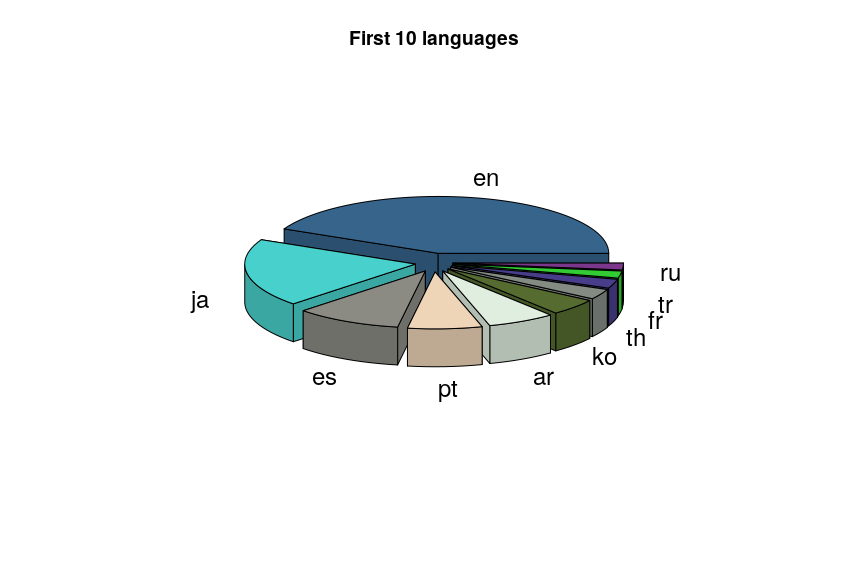
\includegraphics[width=\linewidth]{first_ten_languages.png}}
\caption{Results for 1 208 516 638 tweets analysed (deleted tweet was not count).}
  \label{fig:trump_results}
\end{figure}


\subsection{Pre-processing}
\label{subsub:preprocessing}

In this paper we introduce two new resources for pre-processing twitter data \cite{Jianqiang17}, we used some of their ideas like removing URL, as you can see in the repository, an emoticon dictionary is available in Python and we can remove them from any tweets.Unsure and irrelevant label was not used for this classfication \cite{Poddar16} because we think that it is more relevant to detect bots and not adding them into the analyse process rather than put a tag on them and lose time of computation for sentiment analysis. It is powerful because even it is relevant, we can’t take them for computing them after due to a problem of time. Positive, Negative, and Neutral are the three labels for Sentiment Analysis and Joy, Fear, Anger, Surprise and Sadness are the fifth labels for Emotion Analysis. We pre-process all the tweets as follows:
1) We remove all the emoticons
2) We remove all URLs with a regular expression 
3) Replace targets (e.g. “@John”) by also removing them
4) Removing “RT” for most of the tweet, because it doesn’t mean something for the application. 
Tweets in a general way contain a lot of opinions but they are expressed in different ways by users, as they did \cite{Rebecca11} by keeping emoticons. It deals with the preparation that removes the repeated words and punctuations and improves the efficiency the data. Forward other process is doing like converting upper case to lower case. User names and URLs are not important from the perspective of future processing; hence their presence is futile. All usernames and URLs are removed to improve increase the real result. 



\subsection{Machine learning for Emotion and Sentiment classification}
\label{subsub:ml}

In order to predict the feeling (Postive, negative, neutral) and emotion (joy, anger, sadness, fear,surprise) for each tweet, we used 2 methods. They used other label for emotions that we did not 
To determine the feeling of the tweet, we used the TextBlod librairy which provides a simple API of Natural Languge processing and thus allows us to make the sentiment anlysise. For this, Textblob calculates a Polarity rate of -1 to +1 or -1 corresponds to an extremely negative twitch and an extremely positive +1.
To determine the emotion, we had to create our own classification model (classification in English what) with scikit-learn.
To do this we took a tweet dataset that we labalised (after having data cleaned as indicated in the previous paragraph) thanks to indico.
We then transform this dataset into a term document matrix and apply a TF-IDF standardization to evaluate the importance of the term content in each tweet.
Finally we applied a SVM for the classification because like they said \cite{Medhat14}, it is very suitable for text data.
Once the model was extracted, we used it with spark to predict the emotion of all the tweets.

\subsection{Feature Generation}
\label{subsub:featureGeneration}

Take the example of a two-step algorithm, MapReduce will have to perform two jobs:
At the first job:
1.	Read the initial data.
2.	Execute step 1 in a first job.
3.	Save the intermediate result in a distributed way
In the second job:
1.	Read this result
2.	Execute step 2
3.	Save the result in a distributed way.
Spark shares the RDD with the initial data and, by applying step 1, will provide in step 2 a "virtual" intermediate RDD representing the result of step 1 without necessarily immediately rotating the calculation. When the result of step 2 is requested, Spark will combine the calculations required in steps 1 and 2 into one Spark job that will:
1.	Read the initial data
2.	Perform steps 1 and 2, the intermediate result remaining in memory.
3.	Save the result in a distributed way.
Spark thus avoids expensive distributed writing and replay and then only requires the execution of one job (each job having an incompressible structure cost).
When the algorithm has several steps, the time saving becomes considerable!
Two types of operations (In technical terms, Spark calculates a direct acyclic graph of the operations to be performed, like Apache Storm or Apache Tez) can be performed on RDDs: transformations and actions. Transformations return a new "virtual" RDD: nothing is then evaluated or persisted, while the actions evaluate and return a value. After an action, all the previous transformations are then computed (see the repository in the compute folder).

\section{Implementation}
\label{sec:implementation}

We have used the following technologies for many reasons. Hadoop assumes that conventional approaches (consisting of developing ever more powerful centralized systems) have technical and financial limitations. The development of distributed systems consisting of machines or nodes, relatively affordable (commodity hardware) and scaling out is an alternative from a technical and financial point of view because a distributed system comprising tens, hundreds or thousands of nodes will regularly be confronted with hardware and/or software failures. Google has developed the Google File System (GFS), ancestor of the Hadoop Disrelated File System (HDFS) \cite{Baltas17} and The MapReduce Approach. A Hadoop program usually implements both map tasks and reduce tasks. Hadoop is particularly effective for dealing with problems that have one or more of the following characteristics: Volume of data to store or process very important. Need to perform processing on all data (batch rather than transactional, therefore). Heterogeneous data in terms of origin, structure, and format (JSON for example, Tweets collected via any Tweeter API are send in JSON because of the flexibility of this type of object. Several examples are in the repository for interested readers). Execute the tasks of a Hadoop job in parallel, without a pre-established order. A Hadoop cluster is made up of tens, hundreds, or thousands of nodes. It is the addition of the storage and processing capacities of each of these nodes which makes it possible to offer a storage space and a computing power yet to handle data volumes of several To or Po. To improve the performance of a read / write cluster, Hadoop’s file management system, HDFS, writes and reads files in blocks of 64 MB or 128 MB. Working on such large blocks maximizes data transfer rates by limiting search time on hard drives (seek time). MapReduce is a programming model designed specifically to read, process and write very large volumes of data. A Hadoop program usually implements both map tasks and reduce tasks those programs are usually divided into three parts: The driver, which runs on a client machine, is responsible for configuring the job and submitting it for execution. The map is responsible for reading and processing data stored on disk. The reducer is responsible for consolidating the results from the map and write them on disk. Naturally, the implementation core use Hadoop for these reasons.

\section{Web application}
\label{sec:web_application}


\subsection{Conception of the DataBase (Web Site)}
\label{subsub:conception_db}

In order to allow quick access to the data on the website at any time, we had to make a lot of pre-payment.
Finally, by budget limitation, we can not offer a database with a very strong capacity of cpu or datawharehouse we can manage peta byte data. The PostgresSQL database is based on a micro instance of 1 CPU and 2 GB of ram.
With this configuration, it is clearly impossible to perform complicated SQL queries such as group by, cost, and other aggregation on 350 million lines.
For this reason, we decided to optimize our database and create a table corresponding to a data item that we want to display. The query is thus done only on indexes, the response time is then very fast (100ms maximum) regardless of the size of the table.
To do this, we had to proceed by step:
1st step:
The first step was to define exactly the data we wanted to display: We selected temporal data (Psychological evolution during the year, for each month, according to the time), as well as trends, better users and best retweets monthly / yearly. We also chose to be able to display the psychological profile for each user (Global psychological evaluation, number of tweet / retweet and evolution over the year).
2nd step:
We coded Spark scripts for each problem to calculate what we wanted to display. All calculation scripts are here\footnote{\url{https://github.com/yannistannier/twitter-sentiment-analysis/tree/master/compute}}. 
3rd step:
Each Spark script returned us an aggregated file as we wanted, we just had to import these files into the corresponding tables taking care to organize our indexes.
For example: to retrieve the psychological evolution of a user, we just have to make a simple SQL query on the table {\itshape user\_stat} with a selection on index (where id = 1656561) and the query we reference in 100ms 12 rows corresponding to each month. The same request with several accreditation operators on the initial table took several minutes to answer us.



\begin{figure}[H]
{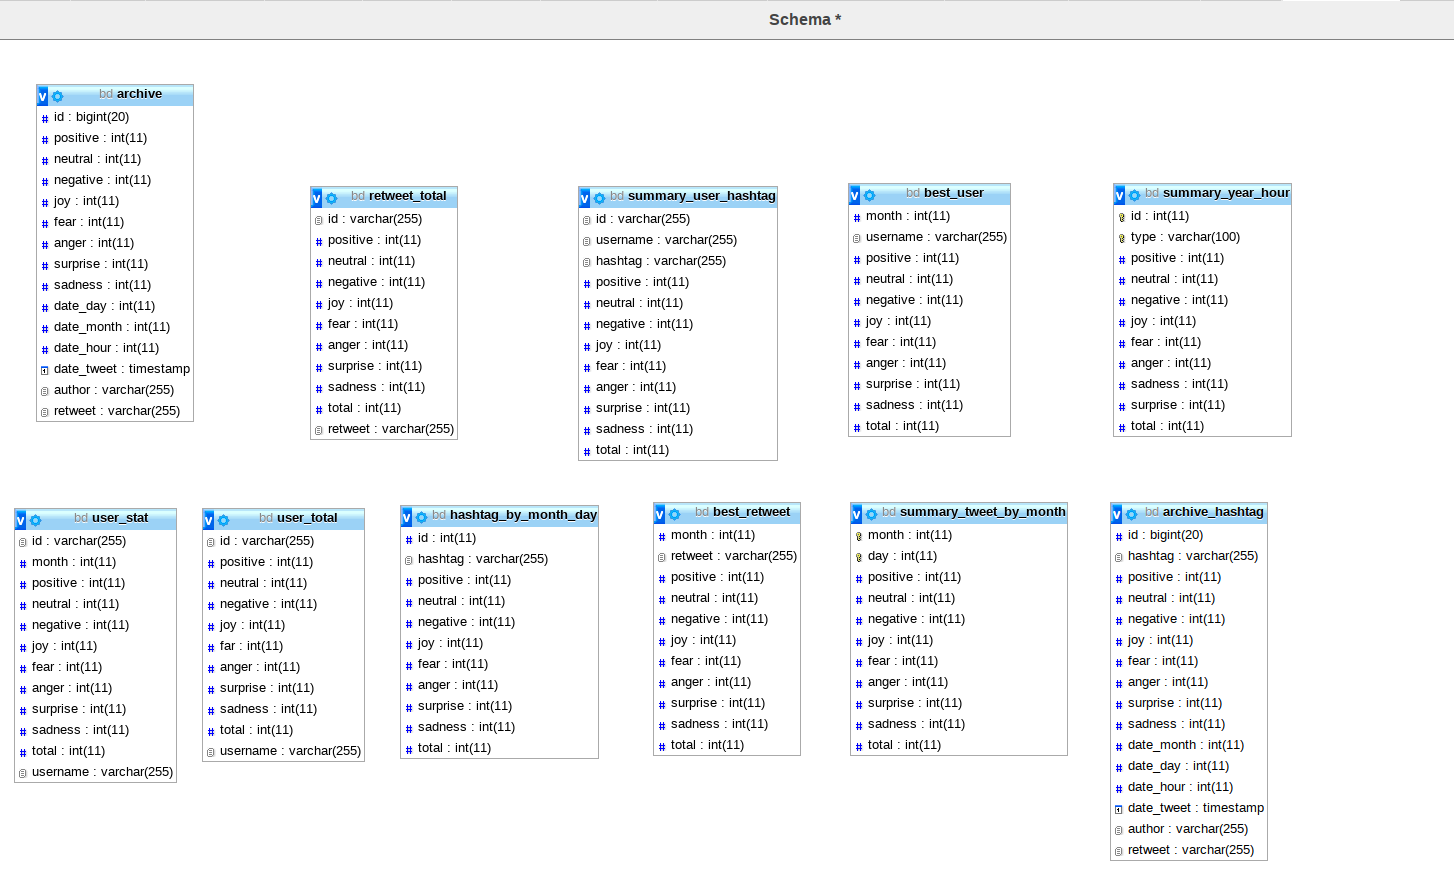
\includegraphics[width=\linewidth]{table-web-db.png}}
\caption{Schema of the DataBase.}
  \label{fig:archivedb}
\end{figure}


\subsection{Conception of the Archive Access}
\label{subsub:conception_aa}

Once the database was created, we wanted the render very easily accessible to the public and we have developed a web platform.
The platform presents a very classic web architecture. Our database Postgres with aggreger data is hosted by AWS RDS.
We have developed Api RestFul through AWS Lambda and AWS GateWey that are responsible for executing sql requests and returning formatting data.
And finally our web client react.js whose sole role is to call the Api Restfull and display the data visualization.


\begin{figure}[H]
{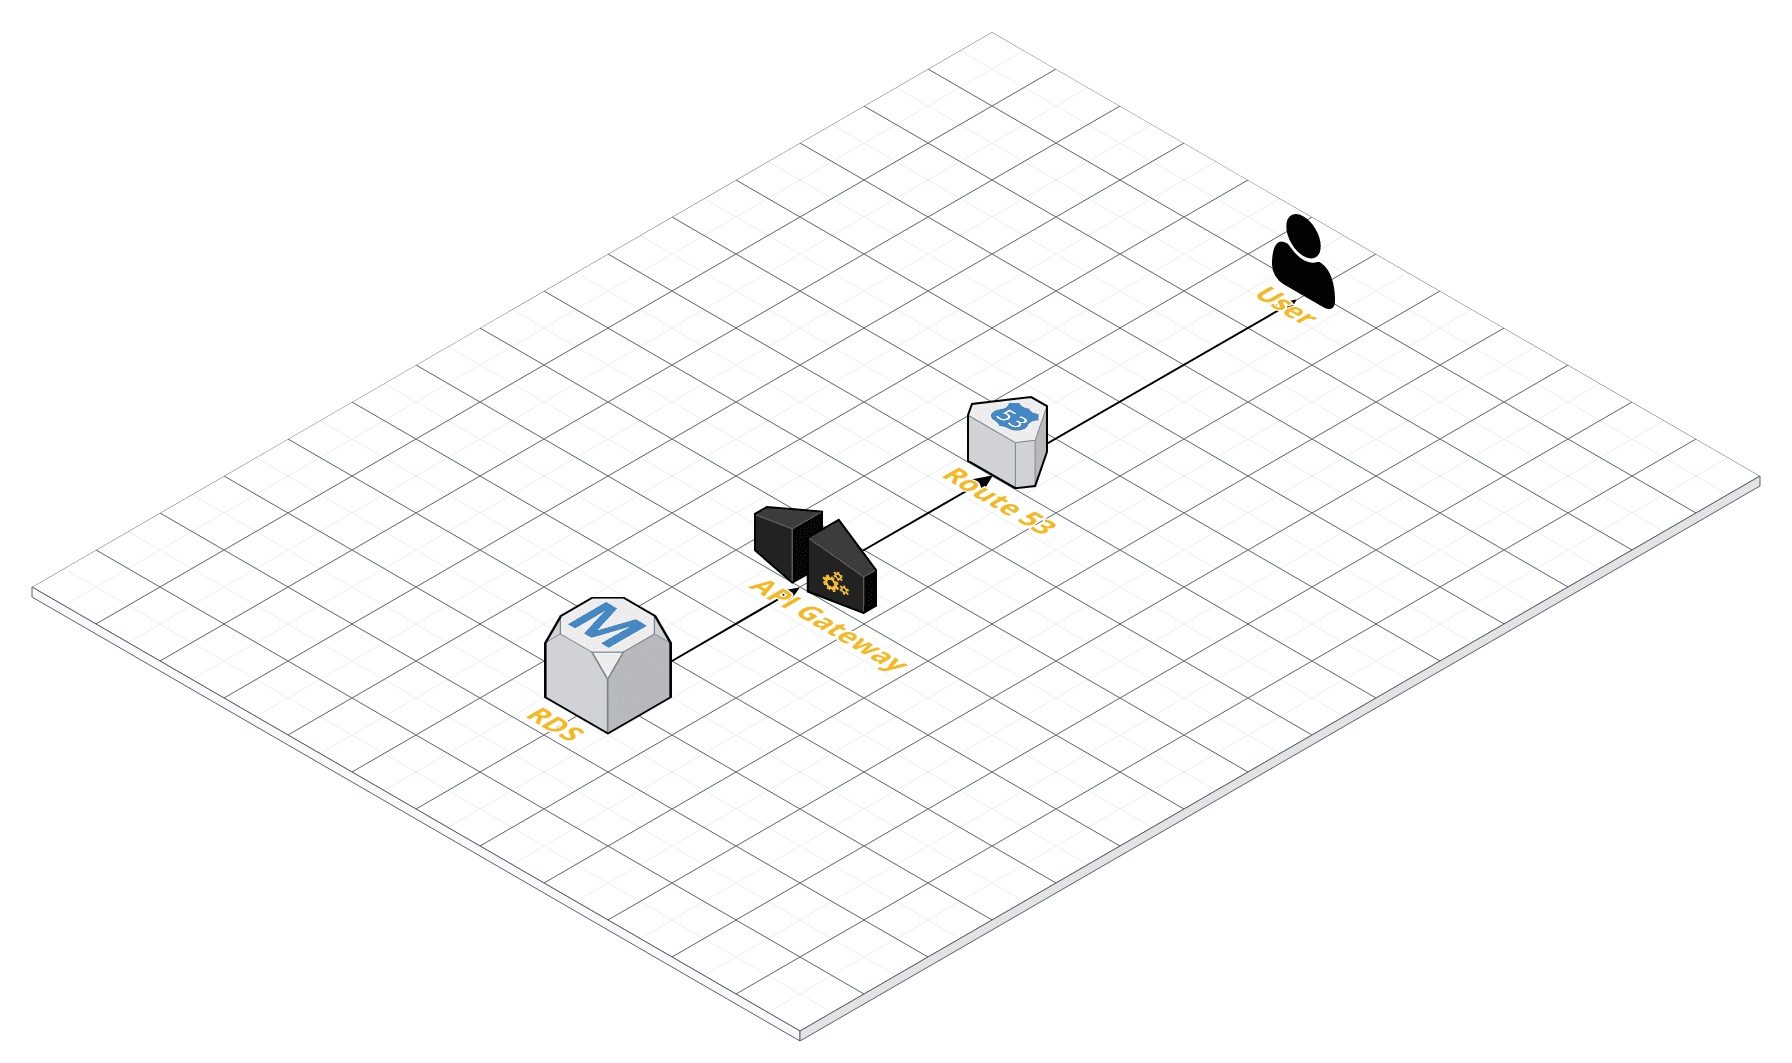
\includegraphics[width=\linewidth]{archive-schema.png}}
\caption{Schema for the Archive Web Application.}
  \label{fig:archiveweb}
\end{figure}

\subsection{Conception of the Real Stream}
\label{subsub:conception_rs}

For the real-time part, we chose to use kinesis Data Streams, which is the real-time data analysis service of AWS.
For this we have created a Twitter streamer that is responsible for recovering real-time data via the API Stream of twitter. This data is sent to Kinesis Data Streams which allows you to aggregate data from multiple sources.
These data are thus sent to a consumer who is responsible for analyzing and predicting the emotion and feeling in real time through textblod and our model of emotion prediction.
Once the data is analyzed, our Consumer formats them and sends the result to our web client thanks to MQTT.
Real streams scripts can be found here\footnote{\url{https://github.com/yannistannier/twitter-sentiment-analysis/tree/master/kinesis-realtime}}.
The streamTwitter.py file is our Twitter streamer and the kinesisStream.py file is our Consumer.


\begin{figure}[H]
{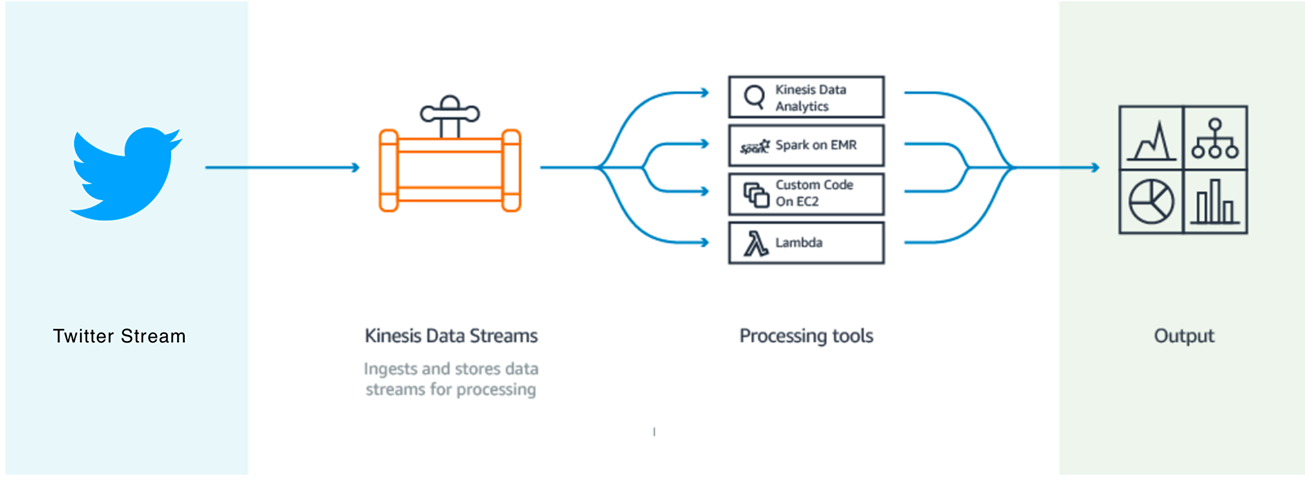
\includegraphics[width=\linewidth]{real_stream-schema.png}}
\caption{Schema for the Real Stream Web Application.}
  \label{fig:archivers}
\end{figure}


\section{Results}
\label{sub:results}

\subsection{English tweets monthly analyzed}
\label{subsub:english_tweets_monthly}

We analyzed the set of English tweets on the year, dividing by month to see any evolution or regression during the year. A thorough American sociological study on the year 2017 could give the reasons for the graph. We were surprised at the symmetry between joy and sadness, proof that the emotional analysis is not as biased as one might think. 


\begin{figure}[H]
{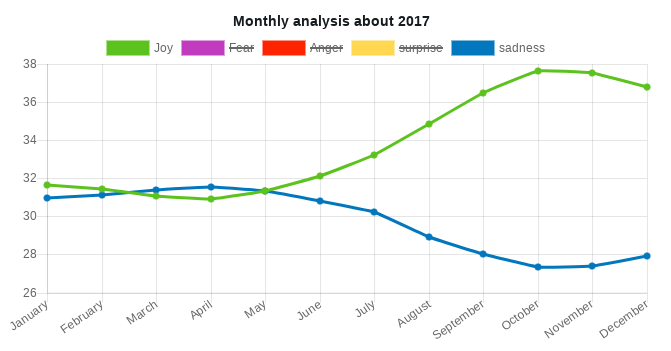
\includegraphics[width=\linewidth]{monthly_analysis_joy_sadness-exemple.png}}
\caption{Results by month for joy and sadness emotions during the 2017.}
  \label{fig:trump_results}
\end{figure}




\subsection{Psychological profile for any users}
\label{subsub:psychological_profile}

We have implemented a psychological profile by current user in the database (note that this feature and also available in the case of streaming too). Here we have taken the case of Donald Trump as an example since he is an active user of the social network. Structure similarity context are a also in search \cite{Zou18}.
The problem of sentiment analysis from archive tweets is that there are not so many tweets as one does not imagine per user.

\begin{figure}[H]
{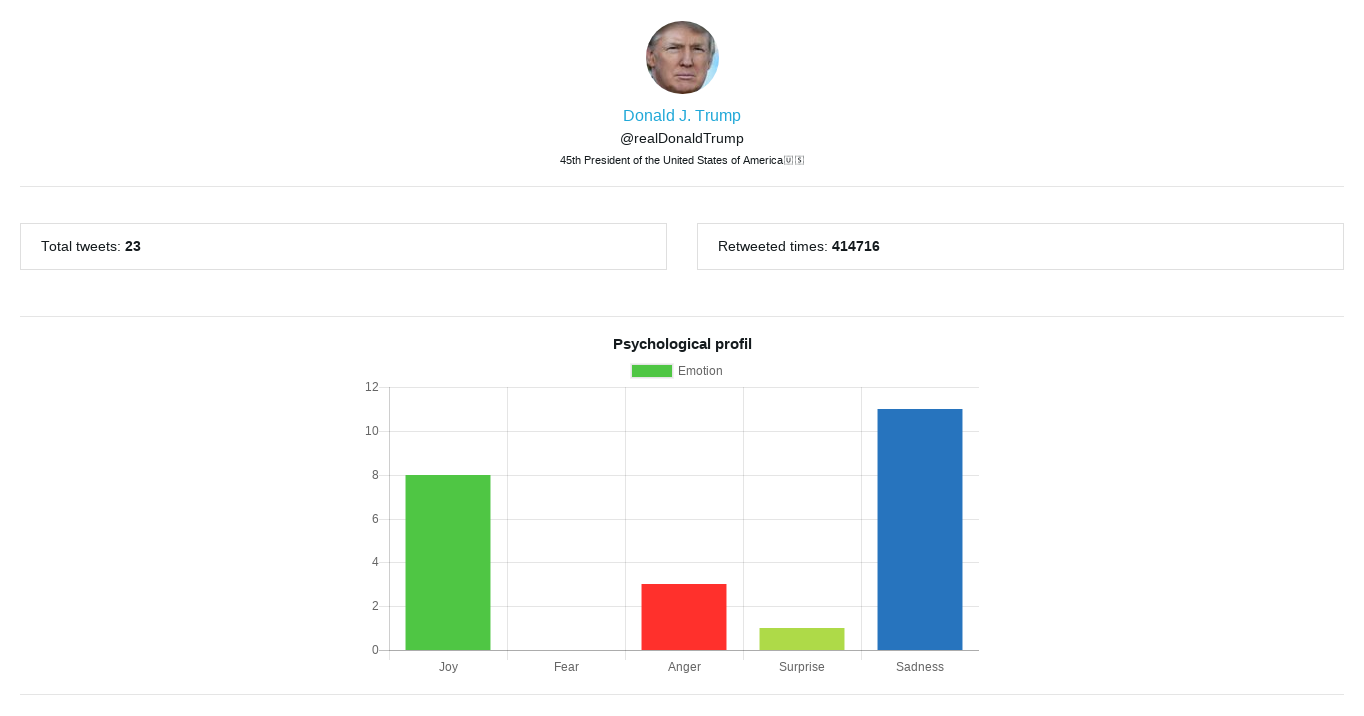
\includegraphics[width=\linewidth]{Trump-results-analysis_exemple.png}}
\caption{Results predicted by our models with Donald John Trump (born June 14, 1946), the 45th and current President of the United States.}
  \label{fig:trump_results}
\end{figure}


\subsection{Impacts of tweets}
\label{subsub:impacts_tweets}

In this section, we wanted to talk about the effect of tweets on the community, taking the utmost retweeting the tweet of Donals Trump. We have 414 716 retweet which allows to have a number of acceptable messages to use the word "impacts". In this publication, \cite{Vyas17}, we found interisting their fought on what they call "influence" and tools used about that. It is interesting in the field of politics but also in the media world to have an analysis of what is said and done in the world today.


\begin{figure}[H]
{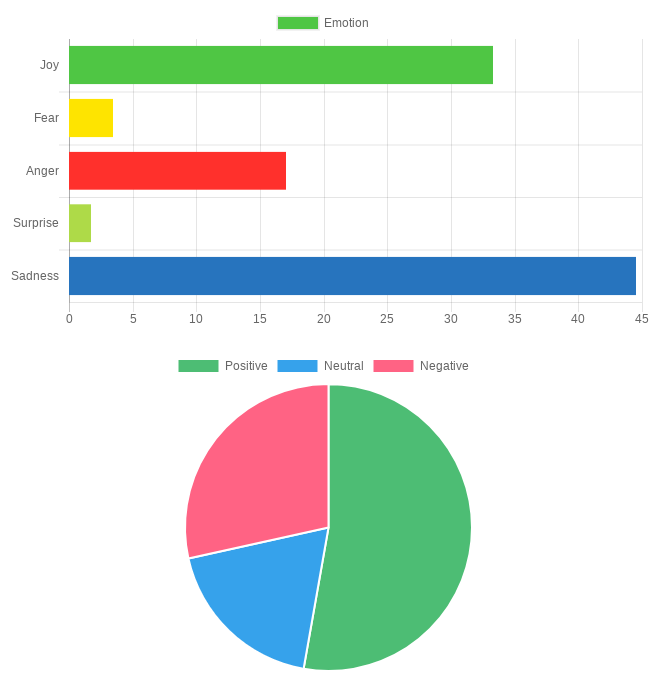
\includegraphics[width=\linewidth]{retweeted_emotion_sentiment_trump-exemple.png}}
\caption{Results for the emotions ratio on the 414 716 retweeted Donald Trump tweets computed.}
  \label{fig:trump_results}
\end{figure}


\section{Discussion}
\label{sec:discussion}

We now turn our attention to the following interesting question: whether the subjective data that exist on the web carry useful information. Information can be thought of as data that reduce our uncertainty about some subject.This is an example with a sample of 383 623 424 tweets in English.

\begin{table}[H]

\tbl{Cross Tab between sentiments and emotions}{%
\begin{tabular}[width=\linewidth]{rcrcrcrcrcrc@{0.5in}}
S\textbackslash E &{Joy} &{Fear} &{Anger} &{Surprise} &{Sadness} \\
$Positive$ & 63 559 579 & 9 296 846 & 27 861 247 & 7 768 707 & 42 382 993  \\
$Neutral$ & 55 127 659 & 15 777 833 & 42 460 015 & 8 879 626 & 48 232 835 \\
$Negative$ & 9 054 496 & 3 395 622 & 23 281 712 & 1 948 578 & 24 595 676 \\
\end{tabular}}
\label{tab:cross_tab}
\end{table}

According to this view, the diversity and pluralism of information on different topics can have a rather negative role. It is well understood, that true knowledge is being described by facts, rather than subjective opinions \cite{ThakkarP15}. However, this diversity in opinions, when analyzed, may deliver new information and contribute to the overall knowledge of a subject matter. This is especially true when the object of our study is the attitude of people. In this case, opinion native data can be useful to uncover the distribution of sentiments across time, or different groups of people. However, data mining differs from machine learning and statistics in that it deals with large volumes of data, stored primarily on disk. Some types of knowledge discovered from a database can be represented by a set of rules. The following is an example of a rule, stated informally: “Donald Trump and his totals of retweets incomes are greater than the average with the most sadly effects on users”. Of course, such riles are not universally true, and have degrees of “support” and “confidence”. Other types of knowledge are represented by equations relating different variables to each other, or by other mechanisms for predicting outcomes when the values of some variables are known. There are a variety of possible types of patterns that may be useful, and different techniques are used to find different types of patterns. Usually there is a manual component to data mining, consisting of preprocessing data to a form acceptable to the algorithms and post-processing of discovered patterns. For this reason, data mining is really a semiautomatic process in real life. The mode widely used applications are those that requires some sort of prediction. In our case, we want to predict emotions and sentiments, then a psychological profile. We outline what is classification, study techniques for building one type of classifiers, called decision-tree classifiers, and then study other predication techniques. Abstractly, the classification problem is this: Given that user in the archive, and given his tweet. We use a given instances of items along with the classes to which they belong, the problem is to predict the class. Since we associate several classes together, then we come to conflicting analyzes. 

\begin{figure}[h!]
{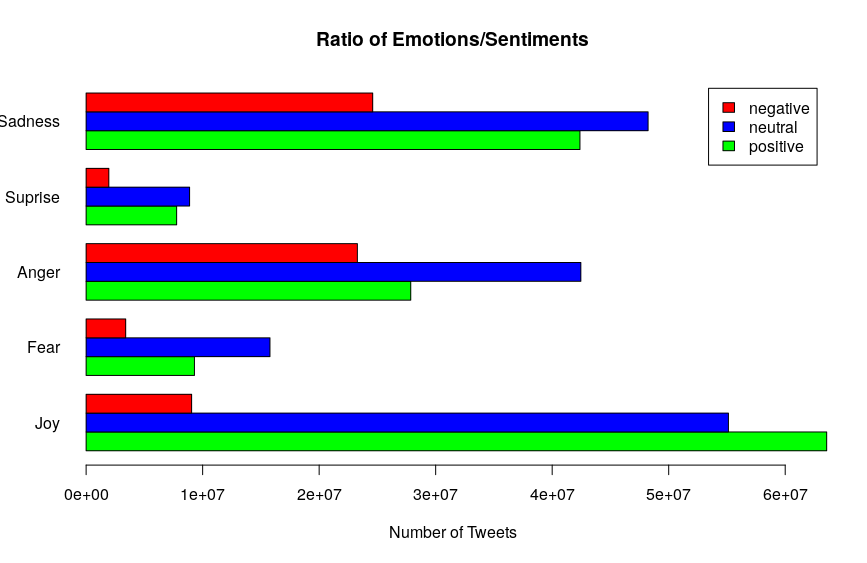
\includegraphics[width=\linewidth]{final_plot_contradiction_analysis.png}}
\caption{Results for ratio Emotion/Sentiment with Number of tweets}
  \label{fig:contradiction_barplot}
\end{figure}

First non-surprising results like Joy/Positive at 49.75 \% and Joy/Negative at 7.08 \%.
We can see that we normally associate sadness with something negative, for example, but here we see that positive feelings are predominant, just as anger has a majority of positive feelings. One publication can also be referred \cite{Alm05}  because accordly to this addition between emotion and sentiment, they also have other results.


\section{Conclusion and Future Work}
\label{sec:conclusion}

In this report we have presented a sentiment analysis tool on a Web interface, in one hand we used data from an archive end in the other we used real time stream analysis. Due to the absence of labelled data we couldn't argue on reliability of data.  This recent publication really question us about the limit on software engineering \cite{Lin18}, but they did not explored deep learning \cite{Meisheri17} and what we could achieve with this learning techniques using neural network fully connected that we always only get better with time because of optimized function behind and great computation that we have nowaydays due to GPU to build deep learning classifier \cite{Araque17}. 
There are also other features for the real stream \footnote{\url{https://twitter.yannistannier.io/#/realtime}} such as geolocation of people, we could then generate a graph as a center to any user and know its impact on an interactive map, this would allow among other things to know the influence for example.

% Start of "Sample References" section

\section{References}

\begin{acks}
We are grateful to the following people for resources, discussions and suggestions: Jason Scott (Archivist) and Diana Yuan (Co-Founder & Vice President, Talent & Operations from Indico).
\end{acks}

% Bibliography

\bibliographystyle{ACM-Reference-Format-Journals}
\bibliography{publication-bibfile}

\end{document}